\section{\trMorseFunction{}的例子}
\label{sec:examples-of-morse-functions}

我们在此给出的那些经典\trMorseFunction{}例子，将在本书中用到。

\subsection{到一点的距离（的平方）函数}
\label{subsec:distance-to-a-point}

正如\cref{subsec:existence-of-morse-functions}所说，函数 $f_p=\|x-p\|^2$ 一般而言是\trMorseFunction。\cref{fig:distance-to-p}展示的，便是这样一个函数在一张\trTorus{}与 $\RR^3$ 中单位\trSphere{}上的两个\trCriticalPoint。

\begin{remark}\label{thm:focal-points-definition}
在\trSphere{}上使 $f_p$ 不成为\trMorseFunction{}的点，只有\trSphere{}的中心。更一般地，我们把 $\RR^n$ 中那些使 $f_p$ 不成为\trMorseFunction{}的点 $p$ 称为 $V$ 的“\textbf{\trFocalPoint}”（focal points）。这一术语的理由在于：在这样的点处（对\trHypersurface{}而言），无限接近的\trNormalVector{}会相遇。倘若把这张\trHypersurface{}想象成一个光源，把\trNormalVector{}想象成它发出的那些光线，那么光强就会在这些点处积聚起来——“\trFocalPoint”之名即由此而来。\footnote{译注：原文此处并列 “foci” 与 “focal points” 两个英文说法，二者同义，中文均译“\trFocalPoint”。}
\end{remark}

\setcounter{figure}{4}%
\begin{figure}[htbp]
\centering
\begin{tikzpicture}[line width=0.6pt]
  \draw[line width=1.1pt] (2.05,1.8) ellipse (1.2 and 0.75);
  \draw[line width=1.1pt] (1.02,1.72) .. controls (1.6,1.3) and (2.7,1.42) .. (3.08,1.98);
  \draw[line width=1.1pt] (1.02,1.72) .. controls (1.45,2.18) and (2.55,2.24) .. (3.08,1.98);
  \draw[dashed] (1.0,2.2) .. controls (1.9,2.68) and (2.9,2.58) .. (3.25,2.15);
  \draw (6.6,1.5) circle (0.78);
  \draw (5.84,1.36) .. controls (6.3,1.0) and (6.95,1.0) .. (7.37,1.4);
  \draw[dashed] (5.84,1.44) .. controls (6.3,1.84) and (6.95,1.84) .. (7.37,1.5);
  \draw (2.68,3.28) .. controls (2.0,2.8) and (1.35,2.54) .. (1.011,2.175)
        .. controls (0.672,1.808) and (0.2,1.25) .. (0.16,0.7)
        .. controls (0.12,0.1) and (0.7,-0.5) .. (1.6,-0.88)
        .. controls (2.6,-1.35) and (4.2,-1.62) .. (7.6,-1.85);
  \draw (0.5,-0.05) .. controls (1.3,-0.75) and (2.6,-1.2) .. (4.2,-1.42)
        .. controls (5.4,-1.52) and (6.3,-1.56) .. (7.2,-1.6);
  \draw[dashed] (3.5,2.88) .. controls (2.9,2.6) and (1.327,2.048) .. (1.02,1.72)
        .. controls (0.713,1.392) and (0.18,1.1) .. (0.18,0.6)
        .. controls (0.18,0.15) and (1.0,-0.25) .. (2.2,-0.5)
        .. controls (3.4,-0.62) and (5.0,-0.66) .. (6.9,-0.66);
  \draw[dashed] (3.95,2.2) .. controls (3.6,2.24) and (3.468,2.208) .. (3.08,1.98)
        .. controls (2.692,1.752) and (2.45,1.4) .. (2.42,1.0)
        .. controls (2.39,0.55) and (2.6,0.05) .. (3.2,-0.37);
  \draw[dashed] (3.95,1.72) .. controls (3.6,1.74) and (3.338,1.605) .. (2.983,1.328)
        .. controls (2.628,1.052) and (2.42,0.72) .. (2.38,0.4)
        .. controls (2.35,0.1) and (2.9,-0.3) .. (3.7,-0.5);
  \draw[dashed] (5.62,1.85) .. controls (5.75,1.5) and (5.809,1.068) .. (6.193,0.834)
        .. controls (6.577,0.6) and (7.3,0.5) .. (8.15,0.62);
  \draw (6.55,2.78) .. controls (6.6,2.6) and (6.623,2.401) .. (7.007,2.166)
        .. controls (7.391,1.932) and (7.52,1.45) .. (7.5,1.0)
        .. controls (7.48,0.62) and (7.9,0.1) .. (8.5,-0.8);
  \fill (4.95,-1.2) circle (1.5pt);
  \node[anchor=west] at (5.05,-1.25) {$p$};
  \node at (2.95,3.42) {极大};
  \node at (3.7,3.02) {\trIndex{} $1$};
  \node at (4.42,2.3) {\trIndex{} $1$};
  \node at (4.3,1.78) {极小};
  \node at (6.42,2.92) {极大};
  \node at (5.5,1.95) {极小};
\end{tikzpicture}
\caption{\trTorus{}与\trSphere{}上的函数“到 $p$ 的距离”}
\label{fig:distance-to-p}
\end{figure}

一般地说，若一张\trSubmanifold{}与过其上一点、以 $p$ 为中心的\trSphere{}相切（非\trTransverse），则该点就是这个距离函数的\trCriticalPoint。

\subsection{\trHeightFunction}
\label{subsec:three-height-functions}

第一部分引言中给出的那三个\trHeightFunction{}都是\trMorseFunction：
\begin{itemize}
\item 在\trSphere{} $S^2$ 上，有两个\trCriticalPoint，\trIndex{}分别为 $0$（极小值，南极）与 $2$（极大值，北极）；
\item 在\trTorus{} $T^2$ 上，有四个\trCriticalPoint：极小值、极大值，以及两个\trIndex{}为 $1$ 的中间\trCriticalPoint；
\item 还是在\trSphere{} $S^2$ 上，有四个\trCriticalPoint：极小值、一个\trIndex{}为 $1$ 的\trCriticalPoint{}和两个局部极大值。
\end{itemize}

\begin{remark}\label{thm:height-distance-infinity}
我们也可以把高度看成到沿 $z$ 轴方向一个无穷远点的距离。
\end{remark}

\subsection{论\trTorus{} $T^2$}
\label{subsec:on-the-torus-t2}

\trTorus{}上还有许多别的\trMorseFunction！例如考虑函数
\[
\begin{array}{rcl}
f\colon\RR^2 & \longrightarrow & \RR\\
(x,y) & \longmapsto & \cos(2\pi x)+\cos(2\pi y)
\end{array}
\]
以及它在\trTorus{} $T^2=\RR^2/\ZZ^2$ 上定义的那个函数——我们仍把它记作 $f$。这是一个乘积函数。\footnote{译注：“乘积函数”（product function）指由因子空间上的单变量函数拼合而成的函数：此处 $f(x,y)=\cos(2\pi x)+\cos(2\pi y)$ 正是把一元函数 $\cos(2\pi\cdot)$ 分别作用到两个圆因子上再相加。}它有四个\trCriticalPoint：
\begin{itemize}
\item 一个极小值，点 $(\frac{1}{2},\frac{1}{2})$；
\item 两个\trIndex{}为 $1$ 的\trCriticalPoint，点 $(\frac{1}{2},0)$ 与 $(0,\frac{1}{2})$；
\item 一个极大值，点 $(0,0)$。
\end{itemize}

\begin{figure}[htbp]
\centering
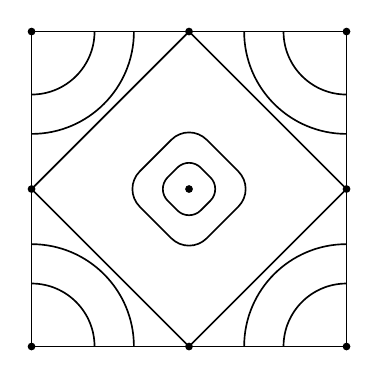
\begin{tikzpicture}[line width=0.6pt]
  \draw (0,0) rectangle (4,4);
  \fill (2,2) circle (1.4pt);
  \draw[rounded corners=6pt] (2,2.42) -- (2.42,2) -- (2,1.58) -- (1.58,2) -- cycle;
  \draw[rounded corners=9pt] (2,2.85) -- (2.85,2) -- (2,1.15) -- (1.15,2) -- cycle;
  \draw (2,0) -- (4,2) -- (2,4) -- (0,2) -- cycle;
  \fill (0,0) circle (1.4pt);
  \fill (4,0) circle (1.4pt);
  \fill (0,4) circle (1.4pt);
  \fill (4,4) circle (1.4pt);
  \fill (2,0) circle (1.4pt);
  \fill (4,2) circle (1.4pt);
  \fill (2,4) circle (1.4pt);
  \fill (0,2) circle (1.4pt);
  \draw (0.8,0) arc (0:90:0.8);
  \draw (1.3,0) arc (0:90:1.3);
  \draw (4,0.8) arc (90:180:0.8);
  \draw (4,1.3) arc (90:180:1.3);
  \draw (0,3.2) arc (270:360:0.8);
  \draw (0,2.7) arc (270:360:1.3);
  \draw (3.2,4) arc (180:270:0.8);
  \draw (2.7,4) arc (180:270:1.3);
\end{tikzpicture}
\caption{\trTorus{}上的一个\trMorseFunction}
\label{fig:torus-morse-function}
\end{figure}

我们请读者验证这些断言（验证过程本身是直截了当的）。\cref{fig:torus-morse-function}描出了\trTorus{}上函数 $f$ 的几个\trLevelSet。注意，极小值位于水平 $-2$ 处，两个\trIndex{}为 $1$ 的\trCriticalPoint{}位于同一水平 $0$ 处，而极大值则位于水平 $2$ 处。
